\begin{abstract} 
The Internet of Things (IoT) makes our lives simple and easier by automating mundane processes with devices around us. Within IoT scenarios, machine-to-machine (M2M) is an inevitable technology that allows machines to own their digital assets and start participating in an economy with other machines, which devices can share and trade their resources. For instance, smart meter data can assist in energy transition. Meanwhile, time smart meter data is privacy-sensitive, that implies power consumption can be associated with appliances used and eventually can be used to track somebody's behavior and location. Questions such as data ownership, data integrity and data privacy become new challenges in M2M economy. In this paper, we leverage usages of distributed ledger technologies (DLTs) to construct an IoT-enabled, decentralized and trusted data marketplace on top of the IoT brokered infrastructure, in order to address the technical challenges. This approach can efficiently enhance the degree of transparency and scalability. The storage via an end-to-end encrypted message streams allows transmitting, accessing and validating data streams over distributed ledgers. Finally, we implement and evaluate the performance of the prototype.
\end{abstract}


Aware of the development of big data science, Radwa et. al.\cite{BigDataaaS} proposed the concept of big data science as a service framework which combines data resources, cloud computing platform and machine learning softwares as building blocks and makes them different subscription services. As more and more platforms and services release, interoperability is arising as a main issue. However, a data trading platform is still the missing piece which data and rewards are traded for innovation. 
 
 
\subsection{choice of data storage}
We assume such storage system should be distributed which runs on the peer-to-peer network maintaining by multiple nodes. Hence, the risk of system paralysis for server being compromised or shutdown unexpectedly can be removed. Among the existing distributed storage mentioned in Section~\ref{section:relatedWork}, different architectures, back-up mechanisms and access controls strategies are proposed. Yet the keys and addresses of data managed by participants are hard to be as small as possible for data streams, and it is difficult to verify arbitrary data pieces, track data streams and categorize.  





% may be removed
The publish-subscribe messaging model is widely used in IoT applications for exchanging data between devices due to its scalability and resource-efficiency. In the publish-subscribe system, a broker is the bridge to meet publishers and subscribers. Broker is a centralized group that arrange the communication between the publishers and subscribers. However, the centralized architecture brings potential vulnerabilities and security issues:

\begin{enumerate}
	\item Central point of failure. 
	The broker is usually held by a single organization. If the centralized server is crashed or attacked, the services will not be available. 	
	\item Data integrity.
	As broker controls the interaction between publishers and subscribers, an unreliable or compromised broker can easily tamper data streams. 
	\item Anonymity and privacy.
	Broker matches publishers and subscribers in order to relay data streams to corresponding entities. The unreliable broker can expose the subscribers' interests and personal information of both entities.  
\end{enumerate}

% move belows to background-archi
The pub/sub model is widely used in IoT applications for exchanging data between devices due to its scalability and resource-efficiency. Connections of participants are built via brokers, which can avert sensitive information leaks in order to establish communication. Yet the existing pub/sub models\cite{MQTT, Looci, centralPubSub} mostly rely on centralized servers which may bring potential vulnerabilities, for instance, the services are paralyzed if the server is crashed or attacked. Therefore, we adopted decentralized pub/sub model with no organization holding brokers. Finally, \textbf{data providers}, \textbf{data consumers} and \textbf{brokers} are the three main roles in the data marketplace.

Ethereum Smart Contract is the key component to enforce the agreement between actors, such as data price and subscription period, and demands penalties when the rules are violated. This stimulates the economics incentives, and motivates data providers to involve data marketplace and maintain high data quality. Also, the interactions among different actors are transparent and validatable by automatically recording them on Ethereum Smart Contracts. 

In our proposed architecture, MAM is the data storage which is the second layer data communication protocol built on top of IOTA\cite{IOTAwhitepaper} network, the Tangle, a feeless cryptocurrency designed for IoT. MAM resolves the challenge of publishing authenticated streaming data as zero-value transactions to distributed ledgers, and provides the ability to publish and fetch encrypted messages over the Tangle along with data integrity and access control. Since the data is zero-value transactions on the Tangle, the concern of losing new uploaded data due to the disconnection does not exist, participants can retrieve the authoraized data streams anytime. 

% MAM performance
optimizing layers of MAM and compare the performance of different cryptosystems. Furthermore, we take offloading MAM operations to brokers as another solution to reduce the workload of IoT devices, since the brokers are considered to have higher computating power. In Section CITE-TA-SECTION, the security issues and methods of offloading will be discussed carefully.

\subsection{Masked Authenticated Messaging}
MAM resolves the challenge of publishing authenticated streaming data as zero-value transactions to IOTA ledger, and provides the ability to publish and fetch encrypted messages over the Tangle along with data integrity and access control. With MAM, the rights of data access is traded instead of a copy of data itself, which eliminates the need for data consumers to have additional storage.
 
In the IOTA protocol, \textbf{seed} is the identifier of its owner. An IOTA seed represents the ownership of all things associated with the user in the IOTA ecosystem, such as IOTA tokens or messages on the Tangle. With the seed, the owner can produce addresses and signatures in order to issue transactions or publish messages to MAM channels and endpoints.

Either channel or endpoint is like a singly-linked list. The MAM channel ID and endpoint ID are the addresses of transaction and are the root of a channel and endpoint. Each address of a message can be derived from the previous one. A user can create multiple channels and multiple endpoints under the same channel. The messages can be encrypted with the session key and broadcasted in chronological order to the Tangle by attaching it to an endpoint. This allows only entities that know the session key to be able to decode these messages after retrieving them from the Tangle, and the singly-linked list structure implements the concept of forward secrecy, where anyone has no access to the data back from his/her entry point. Fig.~\ref{fig:mam_struct} shows the architecture of MAM.

\begin{figure}[!t]
    \centering
    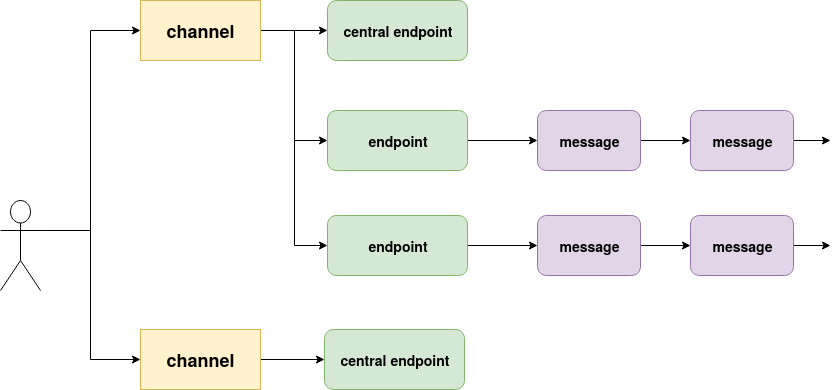
\includegraphics[width=2.5in]{mam_struct}
    \caption{The concept of MAM.}
    \label{fig:mam_struct}
\end{figure}

The authentication in MAM includes source and data authentication. Source authentication ensures that the message originates from the claimed owner, and data authentication ensures the integrity of the data from that sender. These are achieved through the Merkle signature scheme\cite{MSS} (MSS) which is a digital signature scheme based on Merkle Hash Trees and One-way hash functions. However, the size of Merkle Hash Trees should be fixed at start, which is the size of a channel and the endpoint is decided before creation. Thus, data providers need to firstly decide how to distribute data product into MAM channels or endpoints.

%use case illustration
Data providers are the primary role to interact with the MAM. With a seed, a provider can start creating a channel and endpoint. As mentioned above, the length of a channel and an endpoint is fixed, thus providers need to decide the selling unit of data products according to their data type or pricing strategy. Also data providers can a make product preview which is public and not encrypted on MAM. In Fig.~\ref{fig:mam_struct}, a "central endpoint" means its endpoint's ID is the same as channel's ID. By attaching part of the product to central endpoint can give subscribers a quick preview with channel's ID only, and users can easily verify the content with digital signatures in messages. Then if the trade is established, providers can then give subscribers the encrypted endpoint and session key to subscribers.
 
The decentralized and fault-tolerant characteristic of distributed ledgers reduce the risks of centralized storage services, and the underlying IOTA network is scalable which withstands real-time data while increasing users all over the world. Moreover, the features of MAM make it an even better data storage which allows preserving streaming data while ensuring data integrity, proving data ownership to any participants and managing session keys of data. And through the access control and the protocol of MAM, participants are allowed to subscribe to the future data. This ensures that only service requester and selected provider are in possession of a key to decrypt and read the content of the MAM channel and therefore retrieve transaction data for audit.

While the operations of MAM are time-consuming, brokers are responsible not only for being the bridge between providers and subscribers, but also for all MAM related operations, such as channel creation and encrypted data publishing in our system. See Fig.~ \ref{fig:launching_product}.

\begin{figure}[!t]
    \centering
    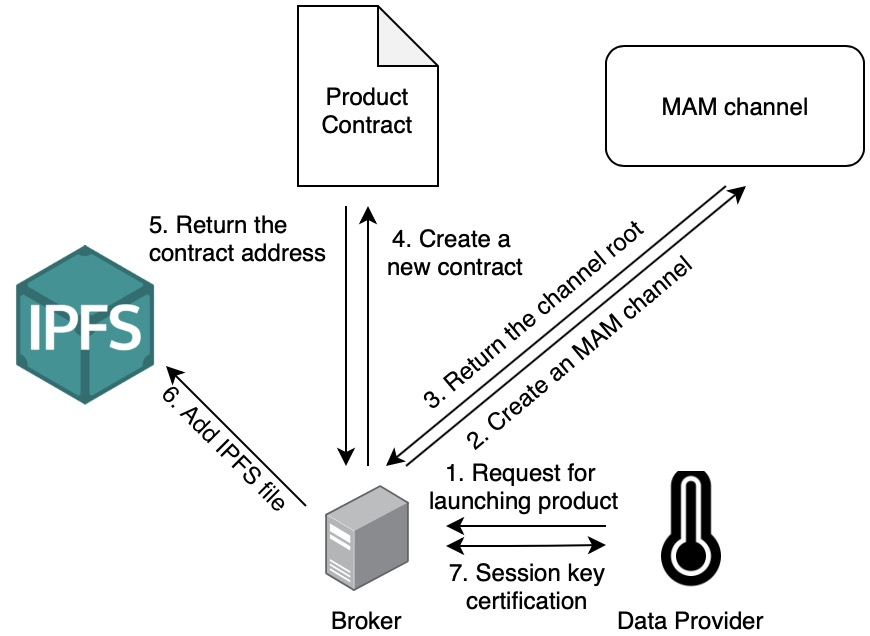
\includegraphics[width=2.5in]{launching_product}
    \caption{The process of launching a product.}
    \label{fig:launching_product}
\end{figure}


\subsection{Components}
There are several building blocks in the proposed design to meet the expectations: 1) emit and access encrypted data stream; 2) retrieve transaction data for audit; 3) digital identity for all participants; and 4) enforcement of transparency and traceability.

